\begin{figure}[H]
\caption{Reactive Streams}
\centering
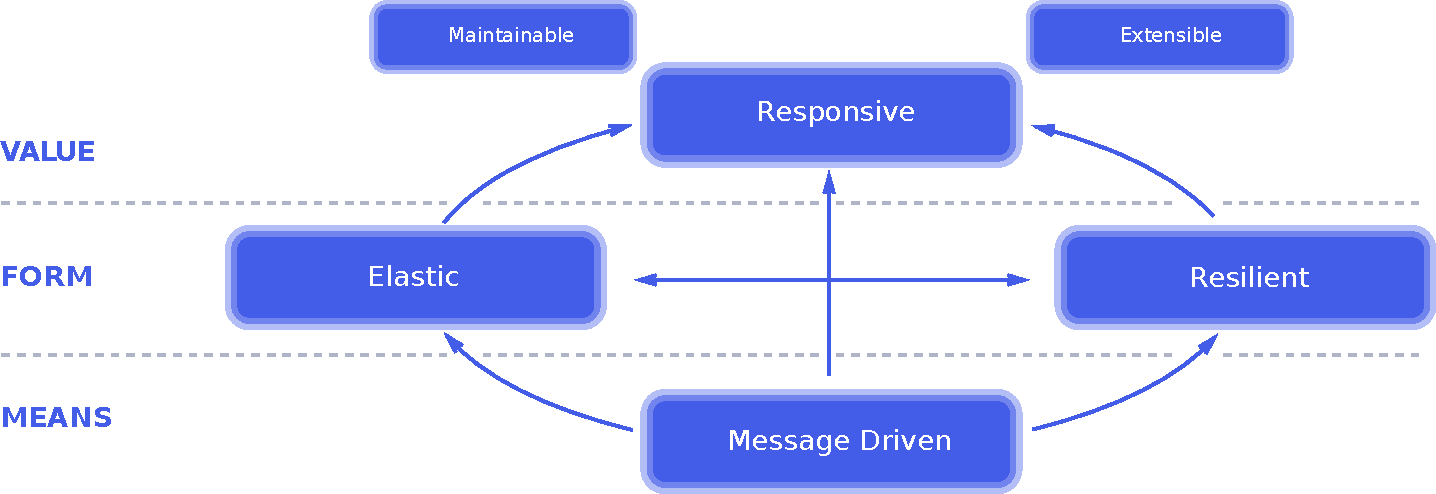
\includegraphics[width=1\linewidth]{images/reactive-traits.pdf}
\small
\textit{Note.} This diagram illustrates the key principles of Reactive Systems as outlined in the \textbf{Reactive Manifesto}. The diagram is divided into three layers: Value, Form, and Means. It showcases six core concepts of Reactive Systems. The layout emphasizes how these concepts interact and support each other.
\textit{Creator.} (\cite{stream})\footnote[34]{\fullcite{stream}}
\end{figure}